In order the classify or train unknown entities, the ed\_perception plugin\footnote{\url{https://github.com/tue-robotics/ed_perception}} exposes ROS Services to classify the entities in the world model. The ed\_perception module interfaces with various image\_recognition nodes that apply state of the art image classification techniques based on \acrfull{cnn} illustrated in Figure \ref{fig:cnn}.
\begin{figure}[H]
    \centering
    %\vspace{-0.3cm}
	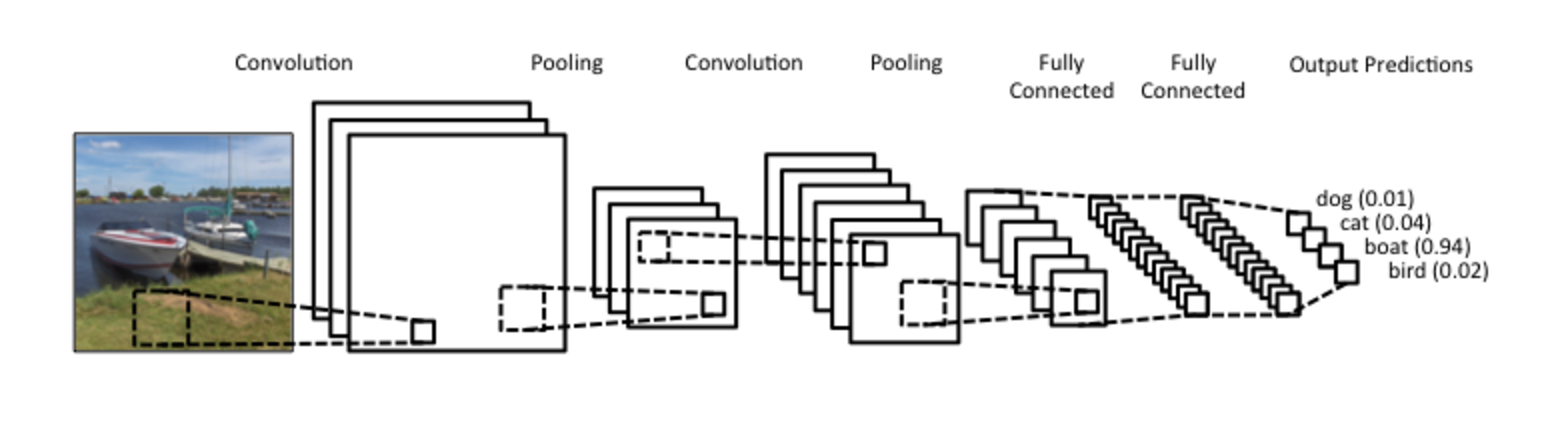
\includegraphics[width = 1\linewidth]{Figures/cnn}
    %\vspace{-1em}
    \caption{Illustration \acrfull{cnn} used in our object recognition nodes with use of Tensorflow.}
	\label{fig:cnn}
    %\vspace{-0.5cm}
\end{figure}

\subsection{Object recognition using Deep Learning}
Object recognition is done using Tensorflow: retraining the top-layer of a Inception V3 neural network. The top layers are retrained on a custom dataset using a soft-max top-layer that maps the image representation on a specified set of labels.
\\
In order to create a new training set for specific objects, the ed\_perception and the image\_recognition packages contains several tools for segmenting and annotating objects. Also tools for retraining neural networks are included.

\subsection{Face recognition}
Face detection and recognition is done using Openface based on Torch. Openface is an existing state-of-the-art face recognition library. We implemented a ROS node that enables the use of these advanced technologies within the ROS network.
\subsection{ROS packages}
Our image recognition ROS packages can be found at GitHub\footnote{\url{https://github.com/tue-robotics/image_recognition}} with tutorials and documentation. Recently, they have also been added to the ROS Kinetic package list and can be installed as Debian packages:
\begin{lstlisting}
ros-kinetic-image-recognition
\end{lstlisting}